\chapter{Base de datos}
\lettrine{E}{n} este capítulo trataremos el diseño de las tablas de base de datos en las que se persistirán los comentarios realizados por los usuarios, así mismo se representarán y describirán todas las entidades relacionadas con los mismos.

\section{Diseño lógico: Modelo Entidad-Relación}
A continuación, se muestra el modelo ER del sistema de comentarios. En este diagrama (fig. \ref{erDiag}) se representan las relaciones y atributos de las 3 entidades utilizadas en subsistema de comentarios: Usuario, Comentario y Articulo.

\begin{figure}[ht!]
	\centering
	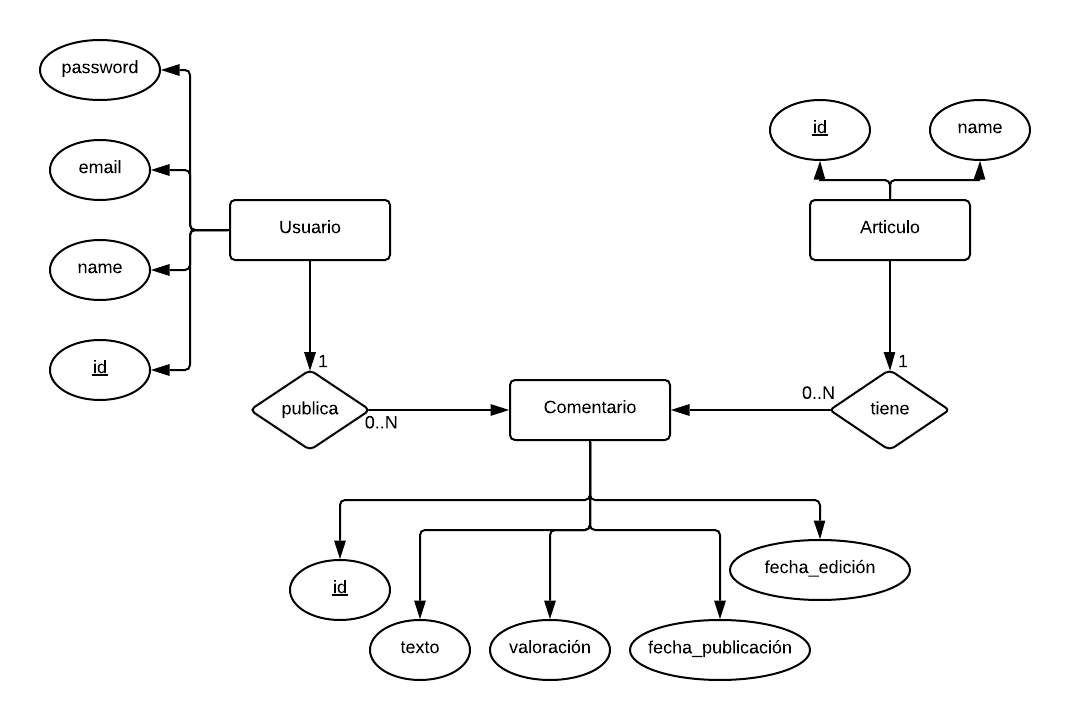
\includegraphics[width=1\textwidth]{imaxes/er.png}
	\caption{Diagrama entidad relación para el subsistema de comentarios.}
	\label{erDiag}
\end{figure}

Siguiendo los requisitos mínimos expuestos por el cliente, un usuario podrá publicar de 0 a N comentarios acerca de un producto, y cada artículo podrá tener 0 o N comentarios.

\section{Diseño físico: Modelo relacional}

La figura \ref{erModel} representa el modelo relacional del subsistema de comentarios.

\begin{figure}[ht!]
	\centering
	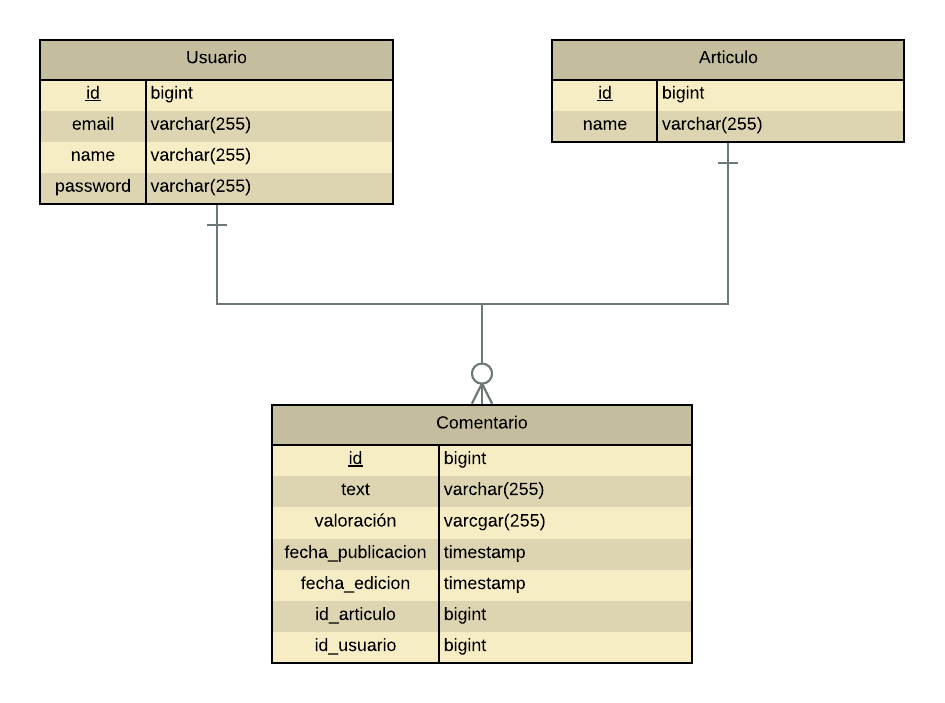
\includegraphics[width=0.75\textwidth]{imaxes/ermodel.png}
	\caption{Modelo relacional para el subsistema de comentarios.}
	\label{erModel}
\end{figure}